\chapter{Introduction}\label{ch:intro}
    \section{Motivation}\label{sec:motiv}
        An example for citation \cite{Hinks2013}. here is an example for abbreviations: \acrshort{gnss} is the abbreviation for \acrlong{gnss}, and this is the full format abbreviation \acrfull{gnss}; \acrshort{gps} is the abbreviation for \acrlong{gps}, and this is the full format abbreviation \acrfull{gps}; \acrshort{leo} is the abbreviation for \acrlong{leo}, and this is the full format abbreviation \acrfull{leo}; 
        
        \lipsum[1]

        An example for figures. 
        \begin{figure}[!ht]
            \centering
            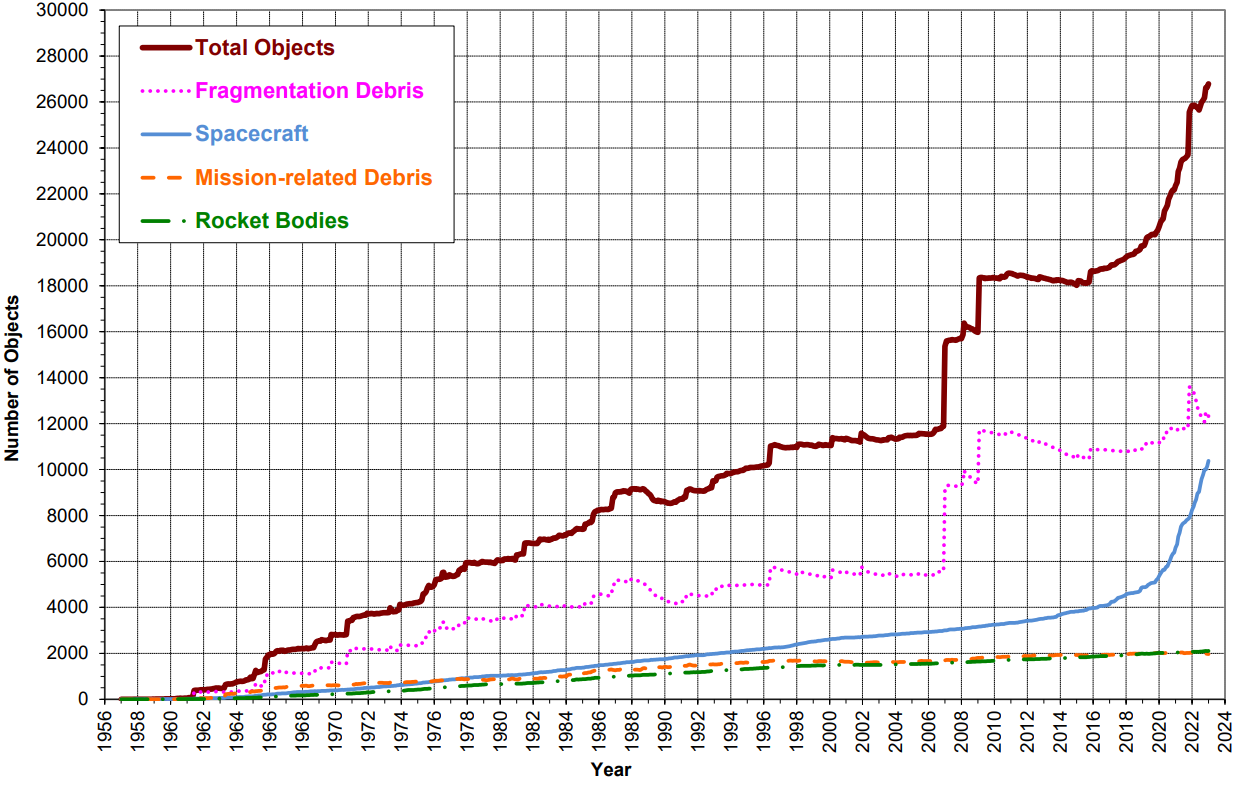
\includegraphics[width=1.0\textwidth]{figures/evo_typ.png}
            \caption{Evolution of number of space objects
            (classified by space object type)\textsuperscript{\cite{nasa2023}}.}\label{fig:evo_typ}
        \end{figure}
        \begin{figure}[!ht]
            \centering
            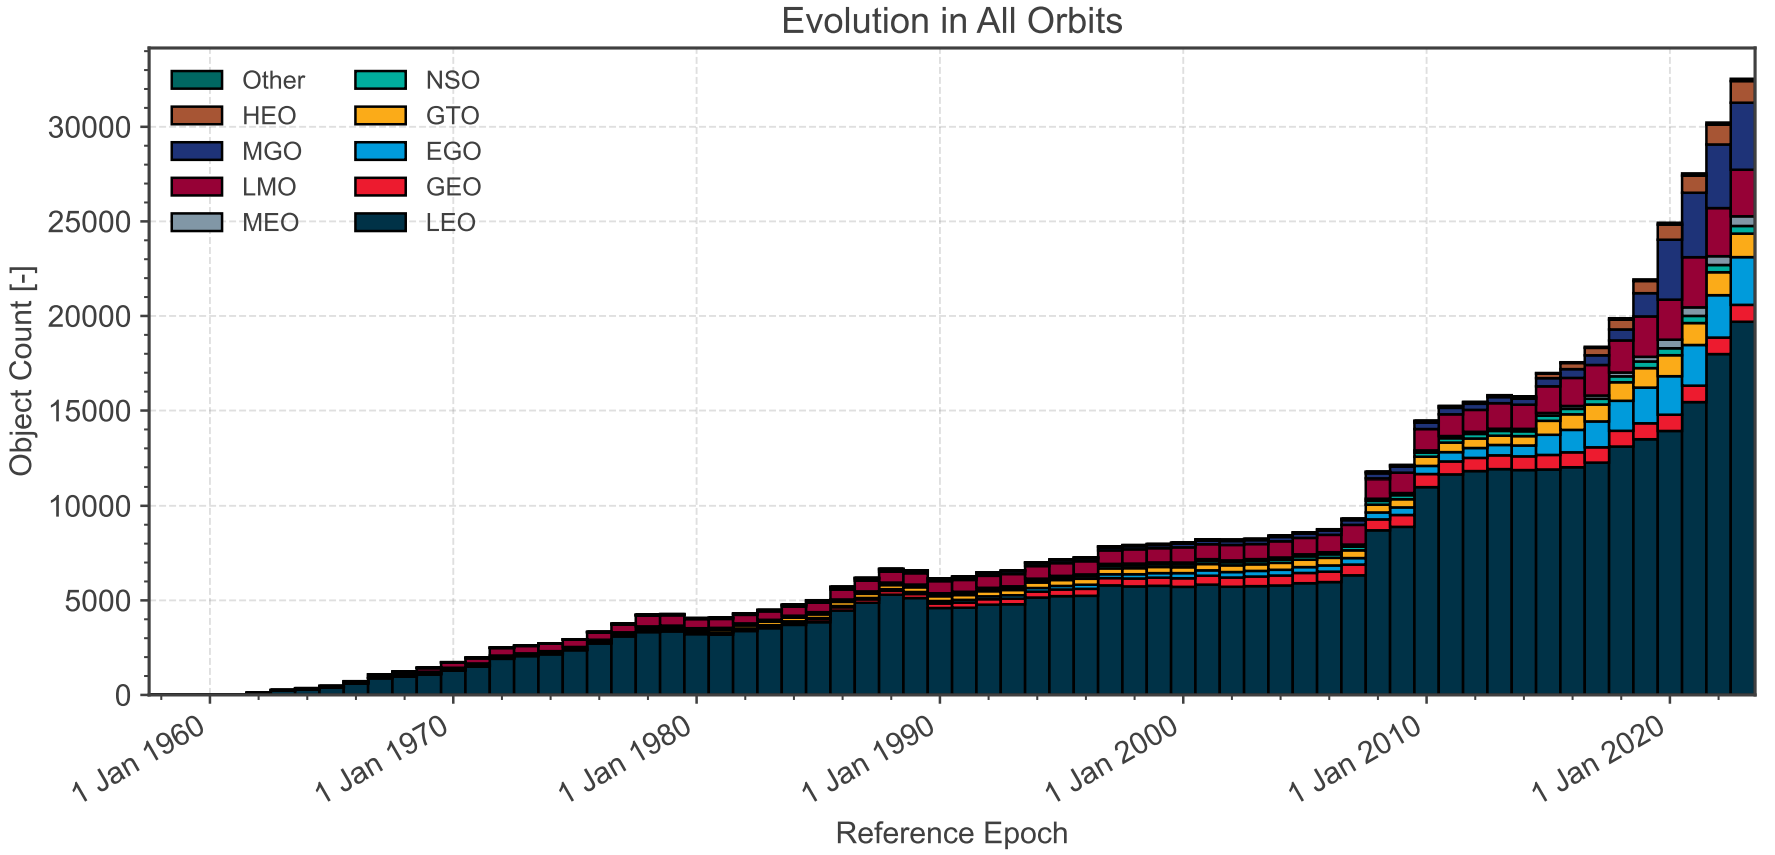
\includegraphics[width=1.0\textwidth]{figures/evo_orb.png}
            \caption{Evolution of number of space objects
            (classified by orbit)\textsuperscript{\cite{esa2023}}.}\label{fig:evo_orb}
        \end{figure}

    \section{Outline}
        Examples for cross references: 

        Chapter \ref{ch:intro} \lipsum[1]

        Chapter \ref{ch:review} \lipsum[1]
        
        Chapter \ref{ch:theory} \lipsum[1]
        
        Chapter \ref{ch:innovation} \lipsum[1]
        
        Chapter \ref{ch:experiments} \lipsum[1]
        
        Chapter \ref{ch:conclu} \lipsum[1]
        
        Chapter \ref{ch:outlook} \lipsum[1]


